% Template for PLoS
% Version 3.1 February 2015
%
% To compile to pdf, run:
% latex plos.template
% bibtex plos.template
% latex plos.template
% latex plos.template
% dvipdf plos.template
%
% % % % % % % % % % % % % % % % % % % % % %
%
% -- IMPORTANT NOTE
%
% This template contains comments intended 
% to minimize problems and delays during our production 
% process. Please follow the template instructions
% whenever possible.
%
% % % % % % % % % % % % % % % % % % % % % % % 
%
% Once your paper is accepted for publication, 
% PLEASE REMOVE ALL TRACKED CHANGES in this file and leave only
% the final text of your manuscript.
%
% There are no restrictions on package use within the LaTeX files except that 
% no packages listed in the template may be deleted.
%
% Please do not include colors or graphics in the text.
%
% Please do not create a heading level below \subsection. For 3rd level headings, use \paragraph{}.
%
% % % % % % % % % % % % % % % % % % % % % % %
%
% -- FIGURES AND TABLES
%
% Please include tables/figure captions directly after the paragraph where they are first cited in the text.
%
% DO NOT INCLUDE GRAPHICS IN YOUR MANUSCRIPT
% - Figures should be uploaded separately from your manuscript file. 
% - Figures generated using LaTeX should be extracted and removed from the PDF before submission. 
% - Figures containing multiple panels/subfigures must be combined into one image file before submission.
% For figure citations, please use "Fig." instead of "Figure".
% See http://www.plosone.org/static/figureGuidelines for PLOS figure guidelines.
%
% Tables should be cell-based and may not contain:
% - tabs/spacing/line breaks within cells to alter layout or alignment
% - vertically-merged cells (no tabular environments within tabular environments, do not use \multirow)
% - colors, shading, or graphic objects
% See http://www.plosone.org/static/figureGuidelines#tables for table guidelines.
%
% For tables that exceed the width of the text column, use the adjustwidth environment as illustrated in the example table in text below.
%
% % % % % % % % % % % % % % % % % % % % % % % %
%
% -- EQUATIONS, MATH SYMBOLS, SUBSCRIPTS, AND SUPERSCRIPTS
%
% IMPORTANT
% Below are a few tips to help format your equations and other special characters according to our specifications. For more tips to help reduce the possibility of formatting errors during conversion, please see our LaTeX guidelines at http://www.plosone.org/static/latexGuidelines
%
% Please be sure to include all portions of an equation in the math environment.
%
% Do not include text that is not math in the math environment. For example, CO2 will be CO\textsubscript{2}.
%
% Please add line breaks to long display equations when possible in order to fit size of the column. 
%
% For inline equations, please do not include punctuation (commas, etc) within the math environment unless this is part of the equation.
%
% % % % % % % % % % % % % % % % % % % % % % % % 
%
% Please contact latex@plos.org with any questions.
%
% % % % % % % % % % % % % % % % % % % % % % % %

\documentclass[10pt,letterpaper]{article}
\usepackage[top=0.85in,left=2.75in,footskip=0.75in]{geometry}

% Use adjustwidth environment to exceed column width (see example table in text)
\usepackage{changepage}

% Use Unicode characters when possible
\usepackage[utf8]{inputenc}

% textcomp package and marvosym package for additional characters
\usepackage{textcomp,marvosym}

% fixltx2e package for \textsubscript
\usepackage{fixltx2e}

% amsmath and amssymb packages, useful for mathematical formulas and symbols
\usepackage{amsmath,amssymb}

% cite package, to clean up citations in the main text. Do not remove.
\usepackage{cite}

% Use nameref to cite supporting information files (see Supporting Information section for more info)
\usepackage{nameref,hyperref}

% line numbers
\usepackage[right]{lineno}

% ligatures disabled
\usepackage{microtype}
\DisableLigatures[f]{encoding = *, family = * }

% rotating package for sideways tables
\usepackage{rotating}

% Remove comment for double spacing
%\usepackage{setspace} 
%\doublespacing

% Text layout
\raggedright
\setlength{\parindent}{0.5cm}
\textwidth 5.25in 
\textheight 8.75in

% Bold the 'Figure #' in the caption and separate it from the title/caption with a period
% Captions will be left justified
\usepackage[aboveskip=1pt,labelfont=bf,labelsep=period,justification=raggedright,singlelinecheck=off]{caption}


\usepackage{algorithm}% http://ctan.org/pkg/algorithms
\usepackage[noend]{algpseudocode}% http://ctan.org/pkg/algorithmicx
\usepackage{amssymb,amsmath,amsthm,amsfonts}

\makeatletter
\let\OldStatex\Statex
\renewcommand{\Statex}[1][3]{%
  \setlength\@tempdima{\algorithmicindent}%
  \OldStatex\hskip\dimexpr#1\@tempdima\relax}
\makeatother

\newtheorem{lemma}{Lemma}
\newtheorem{defi}[lemma]{Definition}
\newtheorem{observation}{Observation}[section]
\newtheorem{remark}[lemma]{Remark}
\newtheorem{theo}[lemma]{Theorem}
\newtheorem{theorem}[lemma]{Theorem}
\newtheorem{corollary}[lemma]{Corollary}
\newtheorem{defisec}{Definition}[section]
\newtheorem{lemmasec}[defisec]{Lemma}

% Use the PLoS provided BiBTeX style
\bibliographystyle{plos2015}

% Remove brackets from numbering in List of References
\makeatletter
\renewcommand{\@biblabel}[1]{\quad#1.}
\makeatother

% Leave date blank
\date{}

% Header and Footer with logo
\usepackage{lastpage,fancyhdr,graphicx}
\usepackage{epstopdf}
\pagestyle{myheadings}
\pagestyle{fancy}
\fancyhf{}
\lhead{
\includegraphics[width=2.0in]{PLOS-submission.eps}}
\rfoot{\thepage/\pageref{LastPage}}
\renewcommand{\footrule}{\hrule height 2pt \vspace{2mm}}
\fancyheadoffset[L]{2.25in}
\fancyfootoffset[L]{2.25in}
\lfoot{\sf PLOS}

%% Include all macros below

\newcommand{\lorem}{{\bf LOREM}}
\newcommand{\ipsum}{{\bf IPSUM}}

\renewcommand{\figurename}{Fig.}

%% END MACROS SECTION

\begin{document}
\vspace*{0.35in}

% Title must be 250 characters or less.
% Please capitalize all terms in the title except conjunctions, prepositions, and articles.
\begin{flushleft}
{\Large
\textbf\newline{Converting a network into a small-world network: A fast algorithm for minimizing average path length through link addition}
}
\newline
% Insert author names, affiliations and corresponding author email (do not include titles, positions, or degrees).
\\
Max Ward\textsuperscript{1,*} and
Amitava Datta\textsuperscript{1}
\\
\bigskip
\bf{1} Computer Science and Software Engineering, University of Western Australia, Perth, WA, Australia
\\
\bigskip

% Use the asterisk to denote corresponding authorship and provide email address in note below.
* max.ward-graham@research.uwa.edu.au

\end{flushleft}
% Please keep the abstract below 300 words
\section*{Abstract}
The average path length in a network is an important parameter for measuring the 
end-to-end delay for message delivery. The delay between an arbitrary pair of nodes 
is smaller if the average path length is low. It is possible to reduce the average
path length of a network by adding one or more additional links between pairs of nodes.
However, a na\"ive algorithm is often very expensive for determining which additional link 
can reduce the average path length in a network the most. In this paper, we present 
an efficient algorithm to minimize the average network path length by link addition.  
Our algorithm can process significantly larger networks compared to the na\"ive 
algorithm. We present a simple implementation of our algorithm, as well as a performance 
study of it in this paper.  


\linenumbers

\section*{Introduction}
Many real-world networks are modeled as a graph, $G=(V,E)$, where $V$ is a set of vertices  
and $E$ is a set of edges connecting some of the vertex pairs from the set $V$. Any message sent 
from a source to a destination propagates through intermediate vertices.  
A packet incurs {\em end-to-end delay} if it has to go through many 
intermediate hops. Since any pair of nodes can act as a source-destination pair, it is desirable 
that all paths in a network go through as few intermediate hops as possible. In other words, 
any traffic in the network will incur less average delay if the average path length 
in the network is low. Quite often the edges of these graphs are considered to be weighted, 
the weights may indicate the cost of establishing an edge, the latency or other factors 
depending on the context of the network.  

Many networks have regular structures, meaning each node is connected to an equal number 
of nodes on an average. This makes the average path lengths in real-world networks quite long. 
In {\em small-world} networks the degree distribution of the nodes follows a power law 
and the average distance between any pair of nodes is usually small. These networks are of  
interest for quite sometime since Milgram's pioneering paper \cite{M}. Watts and Strogatz \cite{WS}
designed an approach that improves the clustering coefficient of a random network and converts 
a random network into a small-world network. Comellas and Sampels \cite{CS} replaced each node of a 
network by a mesh network, the number of nodes in the mesh is equal to the 
degree of the node that is replaced
by the mesh. This converted an arbitrary network into a small-world network. Fall \cite{F} showed that 
the addition of a few random edges in a network can reduce the average path length of a network 
significantly. Lu {\em et al.} \cite{LSG} showed that an arbitrary network can be made into a 
small-world network by introducing a scale-free distribution of nodes in a binary tree network.
 

The small-world nature of a network can be characterized in several different ways. 
However, our focus in this article is the average path length for all pairs of nodes.  
Usually a lower average 
path length reduces the overall communication cost in a network. 
Though there is strong evidence from previous work by Fall ~\cite{F} that addition of extra 
edges can reduce the average path length in a network, the algorithmic nature of this problem 
has been studied only recently. 

Meyerson and Tagiku \cite{MT} have shown that the general problem of adding $k$ edges for minimizing 
the weighted average shortest path lengths between all pairs of vertices is NP-complete. They designed 
several approximation algorithms for this problem \cite{MT}. We are 
interested in this paper in designing an algorithm that adds a single edge to an existing network 
for minimizing the average shortest path lengths between every pair of vertices. Though it may 
seem quite a restricted problem, it has applications in many different areas. Chang {\em et al.}
\cite{CCKN,CSTC} have considered the problem of adding radio-frequency (RF) links in multi-core processor 
design. Their aim is to reduce the latency of communication in multi-core architectures, by adding 
extra radio frequency links on top of a regular interconnection scheme like a mesh network. However 
RF interconnects require much more area and cannot replace the traditional interconnects. Adding even 
a single RF interconnect can improve latency significantly \cite{CCKN,CSTC}. The weight on 
the link is the area requirement for an RF interconnect in this case. Ogras and Marculescu \cite{OM} 
consider a long range link over a regular mesh network for designing efficient Network-on-Chip (NoC) 
in VLSI design. The length of the long link and the volume of traffic between the nodes are  the weights 
on the links in this case. Pickavet and Demeester 
\cite{PD} have designed heuristic algorithms for link restoration in Synchronous Digital Hierarchy (SDH)
networks. One of the key parts in their four-phase algorithm is local optimization, where they 
try to improve the topology in terms of the spare capacity, by adding an extra link. The weight 
on the link is the spare capacity in this case. Jin {\em et al.} \cite{JGN} and Newman \cite{N} 
have simulated stronger community structures in artificial social networks by link addition. It 
is possible to strengthen a community by adding an extra link between two nodes $v_i$ and $v_j$ 
such that they share a relatively large number of friends. The probability of a link addition 
is the weight on an edge in this case and the probability is determined by counting the number of common 
friends.     

Recently Gaur {\em et al.} ~\cite{GCM} have studied several deterministic link addition strategies 
for converting an arbitrary unweighted and undirected network into a small-world network. They found that 
the best strategy is  
to add an additional (long) link in an arbitrary network to minimize 
the average path length of the network. 
Given a graph $G=(V,E)$, 
Gaur {\em et al.} \cite{GCM} considers an $O(V^2\log V)$ algorithm for the all-pairs 
shortest path algorithm for unweighted and undirected graphs. This algorithm is based 
on Dijkstra's shortest path algorithm and not an original contribution by Gaur {\em et al.} as 
they have stated explicitly in their paper \cite{GCM}. 
There is a possibility of introducing 
$O(V^2)$ new edges in a connected graph. The all-pairs shortest path 
algorithm is run after introducing each new edge and the average path length is computed. 
Hence the all-pairs shortest path algorithm needs to be run $O(V^2)$ time and the overall 
complexity of determining which link addition results in the minimum average path length is 
$O(V^2\times V^2\log V)=O(V^4\log V)$. 

In this paper we present a more efficient algorithm for the problem of introducing a new link 
for minimizing the average path length. Our algorithm, unlike that considered by 
Gaur {\em et al.} \cite{GCM}, works on weighted, directed graphs. Hence our algorithm is more general than 
the algorithm considered by Gaur {\em et al.}\cite{GCM}, and, as we will show, it is also asymptotically faster in the worse-case. We present our algorithm, its time complexity and also 
experimental results in this paper. Our algorithm runs in $O(V^2E+V^3)$ time, which has a 
worst-case time complexity of $O(V^4)$ as opposed to the na\"ive algorithm that takes $O(V^5)$
time for weighted directed graphs.   


% You may title this section "Methods" or "Models". 
% "Models" is not a valid title for PLoS ONE authors. However, PLoS ONE
% authors may use "Analysis" 
\section*{Methods}
\subsection*{An efficient algorithm for link addition that minimizes the average path length}

In general, the shortest path between vertices $v_i$ and $v_j$ is the path that has the minimum sum weight. 
In the simplest case each edge has a unit weight, or is unweighted, and the shortest path is the minimum 
number of edges between $v_i$ and $v_j$. 
The {\em single-source shortest path} (SSSP) algorithm finds the shortest paths between a given 
vertex $v_i$ and 
all other vertices in the graph; and the {\em all-pairs shortest path} (APSP) algorithm finds the shortest paths 
between all pairs of vertices. We refer the reader to the book by Cormen {\em et al.}\cite{CLRS} for a review of 
shortest path algorithms. 
We will use the Floyd-Warshall algorithm as the basis of our new algorithm, as it is known to be one of the most 
efficient algorithms for this problem \cite{CLRS}. Asymptotically faster algorithms are known for sparse graphs, but the Floyd-Warshall algorithm is simple to implement and understand, and has very low constant factors in practice. It should be noted that Floyd-Warshall can be trivially replaced by a faster algorithm in our algorithm.
We refer to the problem of {\em link addition that minimizes the average path length} as the {\em MinAPL} problem 
as in ~\cite{GCM}. A na\"ive application of the Floyd-Warshall algorithm can solve this problem in the following way. 
We first compute the APSP of a graph $G$ by executing the Floyd-Warshall algorithm in $O(V^3)$ time, and compute the 
average path length of $G$. Next, we introduce all possible $O(V^2)$ additional links and compute the average 
path length of the resulting graph by using the Floyd-Warshall algorithm and determine the link whose addition 
minimizes the average path length. This algorithm will take $O(V^2\times V^3)=O(V^5)$ time. We show in this 
paper that it is possible to solve this problem in $O(V^4)$ time resulting in a much faster algorithm. 


\subsection*{A fast algorithm for the MinAPL problem}

We first explain a simple property for the addition of a link in a graph. This property will help us in 
designing the efficient algorithm for the MinAPL problem. The proof of the following lemma can be found in 
the book by Cormen {\em et al.}\cite{CLRS}.

\begin{lemma}
\label{lemma1}
Given a weighted, directed graph $G=(V,E)$ with weight function $w:E\rightarrow R$, let 
$p=v_1, v_2, \dots, v_k$ be a shortest path from vertex $v_1$ to $v_k$. For any $i$ and $j$ 
such that $1\leq i\leq j\leq k$, let $p_{ij}=v_i,v_{i+1},\dots, v_j$ be the subpath of $p$ from vertex $v_i$ to 
vertex $v_j$. Then $p_{ij}$ is a shortest path from $v_i$ to $v_j$. 
\end{lemma}

We denote an edge between two vertices $v_k$ and $v_l$ by $e_{kl}$ and the weight of $e_{kl}$ as 
$w(e_{kl})$. We denote the average shortest path length of $G$ as $APL(G)$.  
For a graph $G=(V,E)$, the main task in the MinAPL algorithm is to add an edge between a pair of vertices $(v_k,v_l)$ 
such that $e_{kl}\not\in E$ (we call such an edge an {\em augmenting edge}) and compute the average shortest path length, $APL(G')$  
for the new graph $G'=(V,E\cup e_{kl})$. Then an edge $e_{pq}\not\in E$ is the solution for 
the minAPL problem when, 

\begin{multline}
APL(G') =\min_{\forall e_{kl}\not\in E} APL(G=(V,E\cup e_{kl}))
~
{where} ~ G' = (V,E\cup e_{pq})
\end{multline}

So the main task in our algorithm is to introduce all the augmenting edges $e_{kl}$ one by one and compute the average 
path length of the resulting graph every time and choose the edge that gives the minimum average path 
length. The heart of our algorithm is the following lemma. We denote the shortest path from vertex $v_i$ 
to $v_j$ as $p_{ij}$, and its weight as $w(p_{ij})$. 

\begin{figure}
\centering
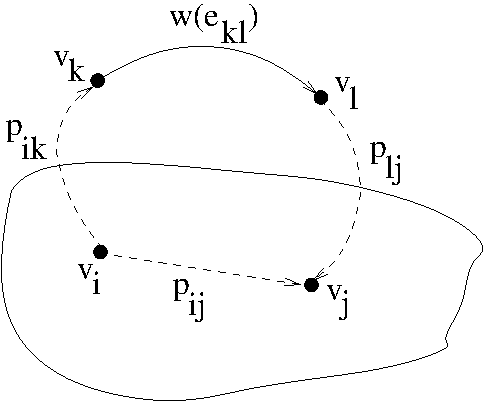
\includegraphics[scale=0.5]{Fig1.pdf}
\caption{Illustration for Lemma \ref{lemma2}.}
\label{algo_fig}
\end{figure}

\begin{lemma}
\label{lemma2}Suppose $G=(V,E)$ is our original graph. 
Consider a directed edge $\overrightarrow{e_{kl}}\not\in E$ and the resulting augmented graph $G'=(V,E\cup e_{kl})$
 after the introduction of $e_{kl}$. 
Consider a pair of vertices $v_i$ and $v_j$. 
The weight of the shortest path from $v_i$ to $v_j$ in $G'$ 
is: $min\{w(p_{ik}))+w(e_{kl})+w(p_{lj}), w(p_{ij})\}$.
\end{lemma}

\begin{proof}
We refer to Fig. \ref{algo_fig} for an illustration. 
Suppose the shortest path from $v_i$ to $v_j$ has changed in $G'$, then this new shortest path must 
go through $e_{kl}$. Also, this new shortest path will consist of the shortest path from $v_i$ to 
$v_k$, $e_{kl}$ and the shortest path from $v_l$ to $v_j$. Note that the difference between the 
graphs $G$ and $G'$ is only in the augmenting edge $e_{kl}$. From Lemma \ref{lemma1}, a subpath of a shortest path 
is a shortest path. Hence $p_{ik}$ and $p_{lj}$ remain the shortest paths in $G'$ between the vertex pairs $(v_i,v_k)$ and 
$(v_l,v_j)$ respectively. So the new shortest path must consist of the weights $w(p_{ik})+w(e_{kl})+w(p_{lj})$,
if  $w(p_{ij})>w(p_{ik})+w(e_{kl})+w(p_{lj})$.
\end{proof}

We can take advantage of Lemma~\ref{lemma2} in the following way. If we compute all-pairs shortest paths 
in the original graph $G$, we have the weights $w(p_{ik})$ and $w(p_{lj})$ that we can use for determining the 
new shortest paths in $G'$ for all vertex pairs like $(v_i,v_j)$. We first run the Floyd-Warshall algorithm on 
the input graph $G$ and store the weights of the all pairs shortest paths in a matrix $ASP$. The entry $ASP[i,j], 1\leq i,j \leq |V|$,
stores the weight of the shortest path from $v_i$ to $v_j$. Note that $ASP[i,j]\not=ASP[j,i]$ in general as 
$G$ is a directed graph. Next we introduce the augmenting edges separately and iteratively and compute the new average path 
length for each augmented graph after the introduction of an augmenting edge. The algorithm outputs the augmenting edge
that minimizes the average path length among all possible augmenting edges. The $ASP$ matrix can be populated 
in $O(V^3)$ time using the Floyd-Warshall algorithm. The average path length of $G$ can 
also be computed at the same time. Our algorithm is stated in 
Algorithm 1.

The correctness of the algorithm follows from Lemma~\ref{lemma2}. Since there are $O(V^2-E)$ augmenting 
edges, the outer for loop executes $O(V^2-E)$ times. The inner for loop examines every edge in $G$, 
hence it executes $O(E)$ times for every iteration of the outer loop, giving an overall complexity of 
$O(V^2E+V^3)$, which is $O(V^4)$ in the worst case. The second term in the complexity is due to the 
complexity of the Floyd-Warshall algorithm that needs to be run before our algorithm. 
The complexity of executing the Floyd-Warshall algorithm 
na\"ively for each augmenting edge will be $O(V^5)$ as stated in the previous section. 

\begin{algorithm}
\label{algorithm1}
\caption{Algorithm  MinAPL}
{\bf Input:} A directed graph $G=(V,E)$ where $w_{ij}$
             is the weight of edge $e_{ij}$ between vertices $v_i$ and $v_j$. and $e_{ij}=\infty$ if there is no edge between $v_i$ and $v_j$.

{\bf Output:} An augmenting edge $e_{kl}$ that minimizes the average shortest path length in $G$.
\begin{algorithmic}
\Function{MinAPL}{$G$}
        \State $ASP, minAPL \gets \textit{Floyd-Warshall(G)}$
        \State $edge \gets \emptyset$
        \ForAll{augmenting edges $e_{kl} \not\in E$}
                \State $sum \gets 0$
                \State $paths \gets 0$
                \ForAll{vertex pairs $v_{i}$, $v_{j}$ in $G$}
                        \State $sp \gets \min(ASP[v_{i},v_{j}],$
                        \Statex[4] $ ASP[v_{i},v_{k}]+w(e_{kl})+ASP[v_{l},v_{j}])$
                        \If{$sp \neq \infty$}
                                \State $sum \gets sum+sp$
                                \State $paths \gets paths+1$
                        \EndIf
                \EndFor
                \State $APL \gets sum/paths$
                \If{$APL < minAPL$}
                        \State $minAPL \gets APL$
                        \State $edge \gets e_{kl}$
                \EndIf
        \EndFor
        \State \Return $edge$
\EndFunction

\end{algorithmic}

\end{algorithm}


% Results and Discussion can be combined.
\section*{Results}

\begin{figure}[!t]
\centering
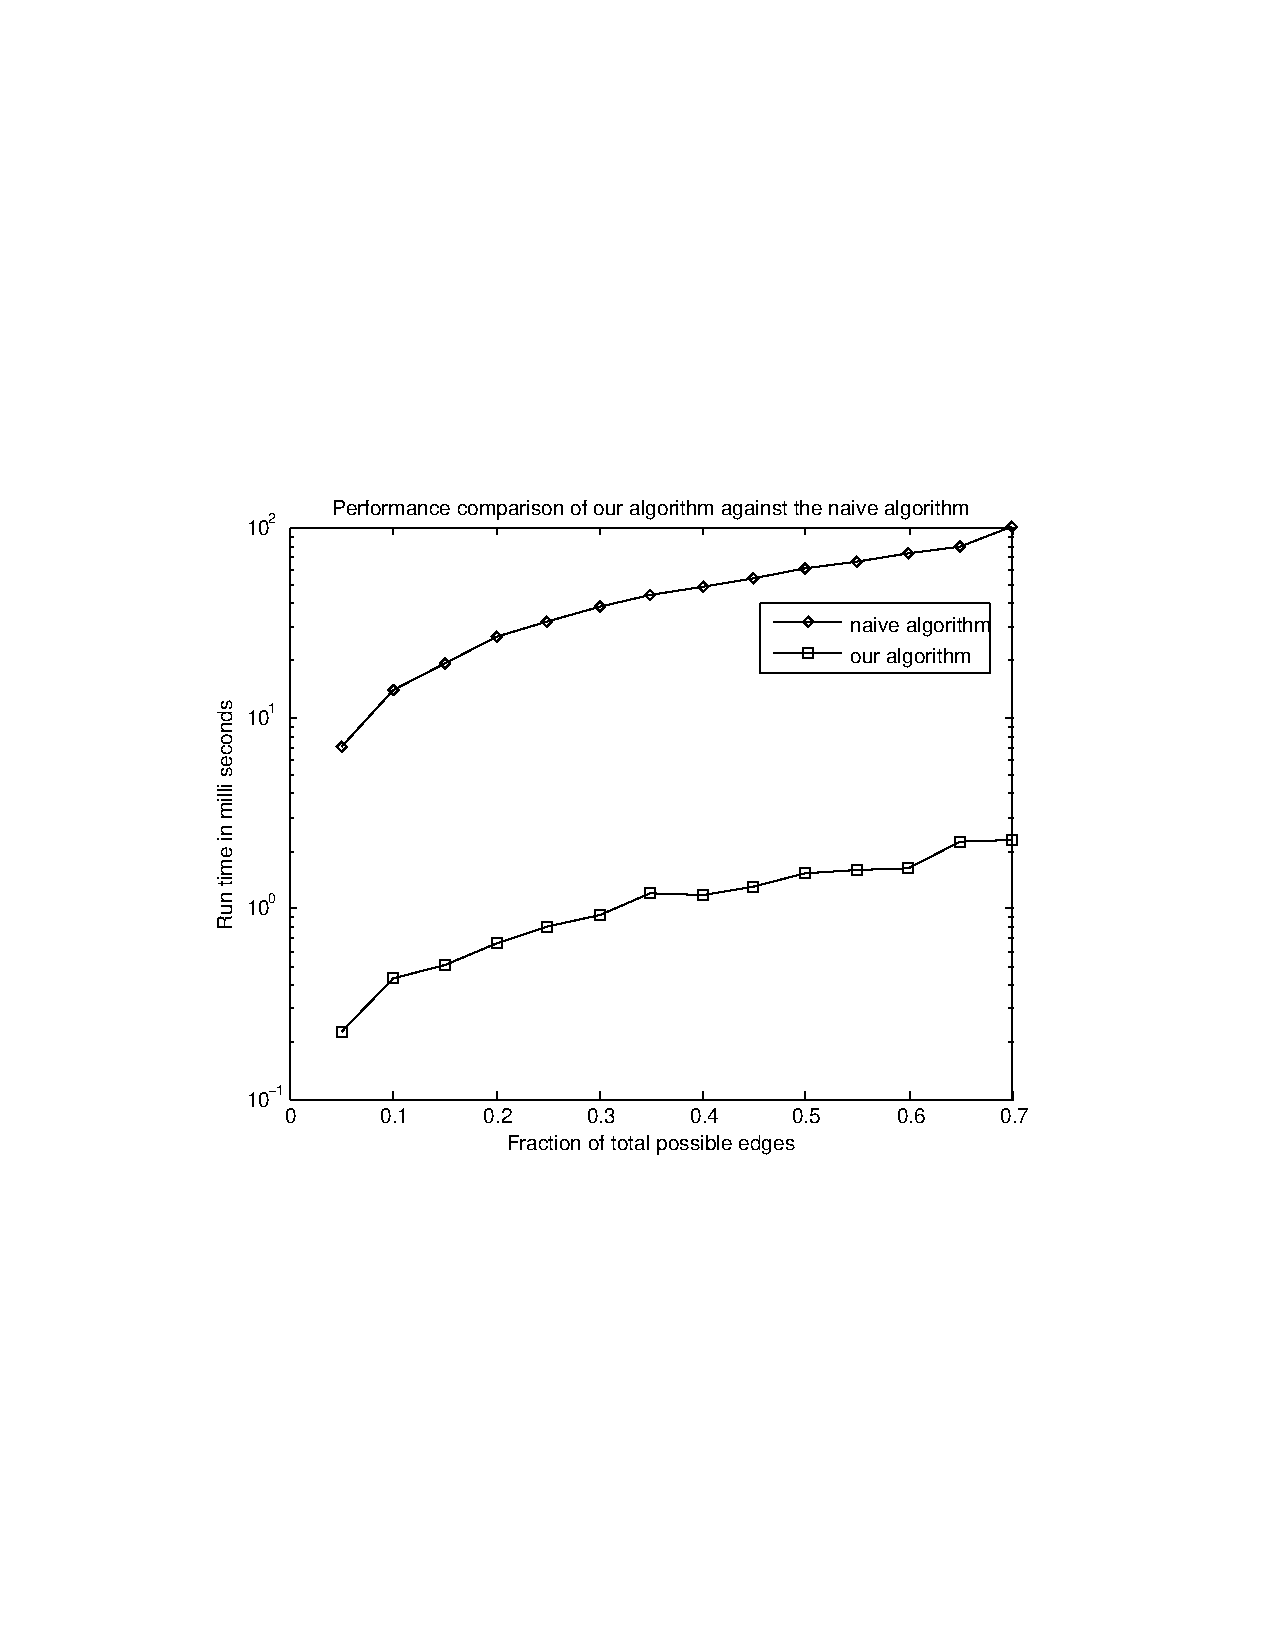
\includegraphics[scale=1.0, width=\columnwidth]{Fig2.pdf}
\vspace{-4cm}
\caption{A comparison between the na\"ive algorithm and our algorithm for graph with $40$ vertices
         and different fraction of the total edges. The runtime is plotted in a logarithmic scale.} 
\label{fig1}
\end{figure}


We have done extensive experiments for evaluating the performance of our algorithm. All experiments 
were run on a Virtualbox Ubuntu 14.04 on an i7 3630QM processor.  The algorithm was implemented using C++ and the GNU C++ compiler. 
For each of the experiments we have ensured that the output of our algorithm matches the output from the 
na\"ive algorithm exactly. 
All our graphs were generated through random introduction 
of edges ensuring that the graph was connected. First we generated random graphs with $40$ vertices 
with different edge densities as a fraction of the total possible edges of the complete graph. The set of augmenting edges was defined as the remaining edges not added to the graph. The 
performance comparison of the na\"ive algorithm with our algorithm is shown in Fig. \ref{fig1}. The weights 
on the edges are randomly generated with a value between $1$ and $100$.
Our algorithm runs much faster for 
both sparse and dense graphs. If the total number of edges for the complete graph is represented as 
$C$, our algorithm runs in less than a milliseconds for $0.3C$ augmenting edges, while the na\"ive algorithm 
runs in about 38 milliseconds. Similarly, for $0.7C$ augmenting edges, our algorithm runs in $2.3$ milliseconds, 
whereas the na\"ive algorithm takes over $100$ milliseconds. Though we have run our algorithm several times for 
each graph, the running times were almost identical for each run and hence we have not shown any confidence intervals 
in the graphs.  

Next, we evaluated the run times of the two algorithms for larger graphs. We fixed the number of augmenting edges to $0.4C$ while increasing the 
number of vertices. The results are shown for the na\"ive algorithm 
and our algorithm in Fig. \ref{fig2}. Our algorithm outperforms 
the na\"ive algorithm significantly in this case as well. For example, the runtime of the two algorithms 
are $46.54$ and $4472.14$ milliseconds respectively for a graph with $100$ vertices. Similarly, for 
a graph with $400$ vertices, the respective runtimes are $11873.8$ and $4.18\times 10^6$ milliseconds 
respectively. 


\begin{figure}[!t]
\centering
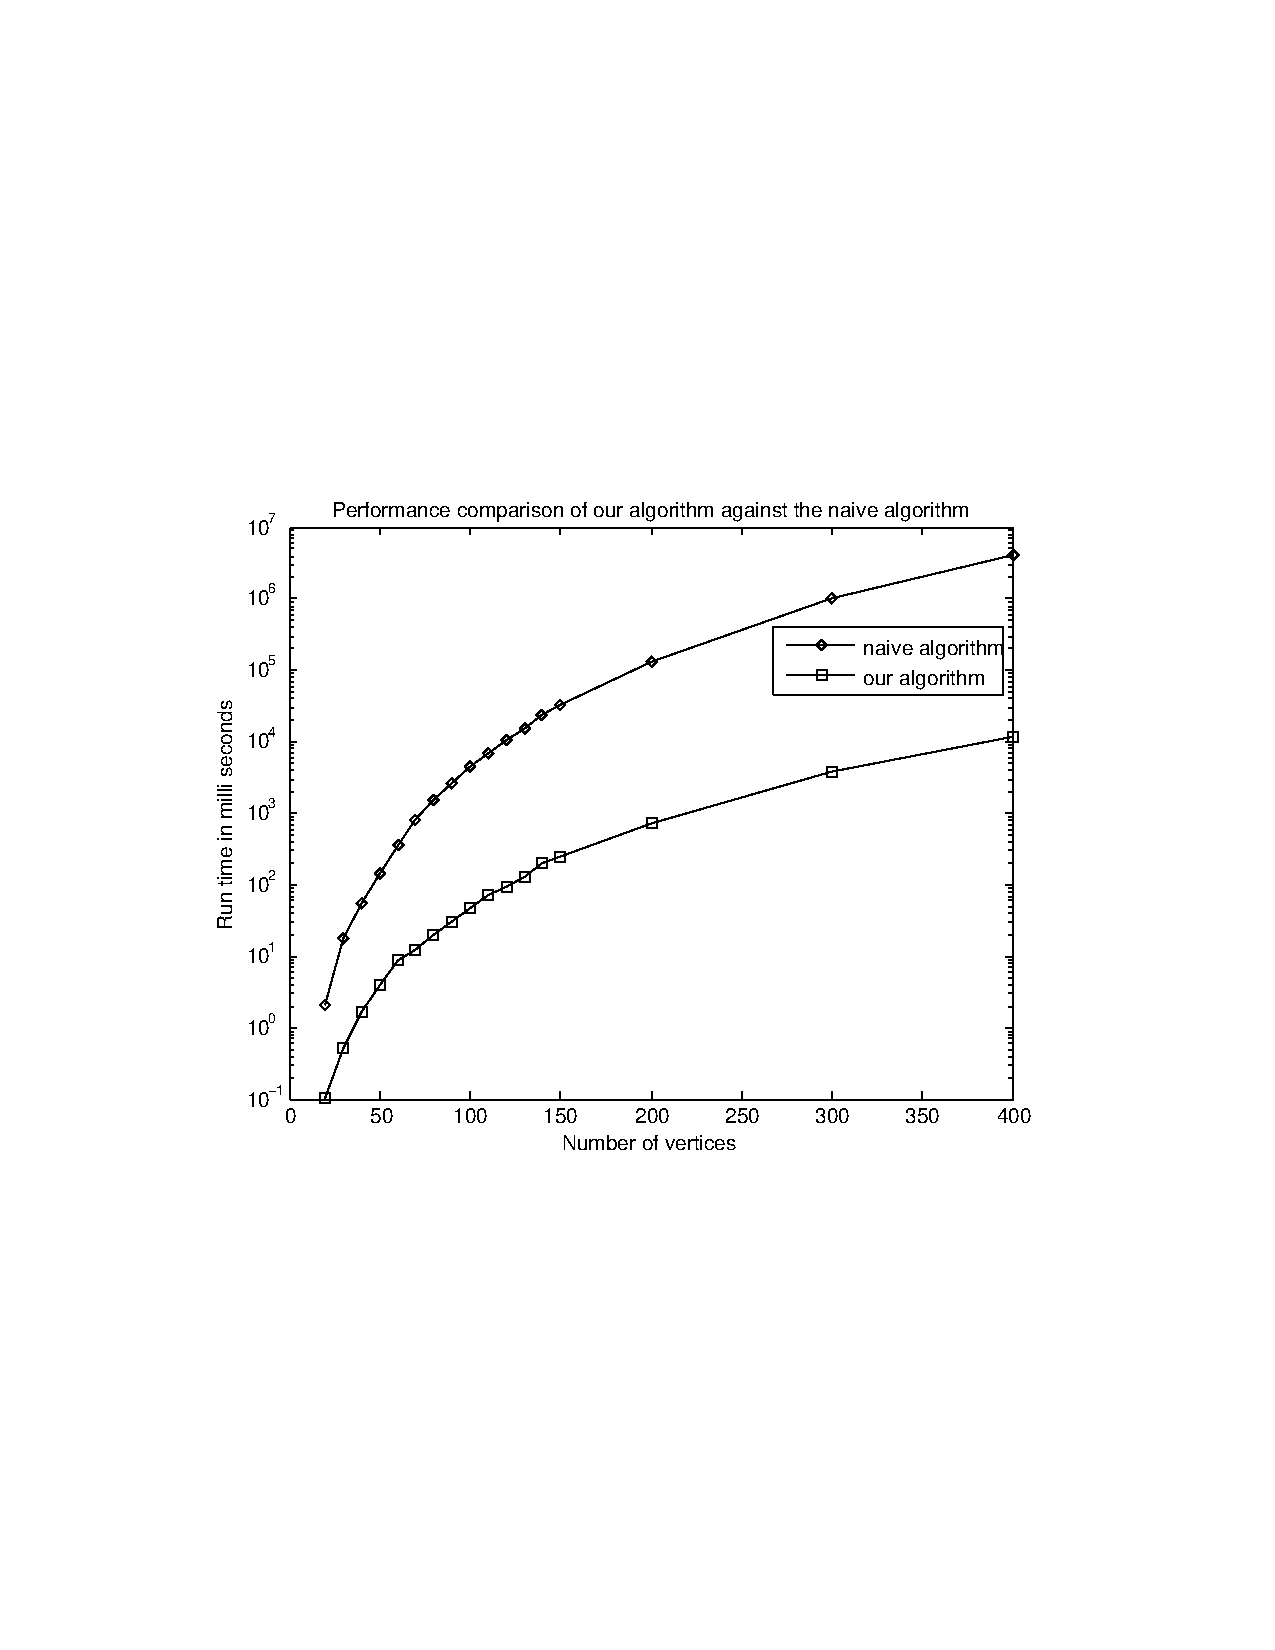
\includegraphics[scale=1.0, width=\columnwidth]{Fig3.pdf}
\vspace{-4cm}
\caption{The performance comparison between our algorithm and the na\"ive algorithm for different
         graph sizes. Each graph has a fraction of $0.6$ of the total edges. The augmenting edge is
         chosen from the remaining fraction of $0.4$ of the total edges. The runtime is plotted
         in a logarithmic scale.}
\label{fig2}
\end{figure}


\section*{Discussion}
We have presented a simple and efficient algorithm for adding an edge in a graph for minimizing the average shortest path length of the graph. The algorithm improves upon the na\"ive algorithm significantly and can be used 
for addition of edges in large graphs for minimizing the average path length. As an example, our algorithm 
finds an augmenting edge that minimizes the average path length of a graph with $1000$ vertices in about 
$7$ minutes.   


\section*{Supporting Information}

% Include only the SI item label in the subsection heading. Use the \nameref{label} command to cite SI items in the text.
\subsection*{Source Code}
\label{S1_Video}
The source code for our algorithm, and the testing framework for it, is available on GitHub. It can be found here \url{https://github.com/maxhwardg/best-link-addition}.

\section*{Acknowledgments}
Cras egestas velit mauris, eu mollis turpis pellentesque sit amet. Interdum et malesuada fames ac ante ipsum primis in faucibus. Nam id pretium nisi. Sed ac quam id nisi malesuada congue. Sed interdum aliquet augue, at pellentesque quam rhoncus vitae.

\nolinenumbers

%\section*{References}
% Either type in your references using
% \begin{thebibliography}{}
% \bibitem{}
% Text
% \end{thebibliography}
%
% OR
%
% Compile your BiBTeX database using our plos2015.bst
% style file and paste the contents of your .bbl file
% here.
% 


\bibliography{edge_addition}


\end{document}

